\subsection{Injections}

In this chapter you will learn how to implement methods that you cannot express as SDMs by adding handwritten code to classes created from your model.

Injections are inspired by partial classes in C\#, and are our preferred way of providing a clean separation of generated from handwritten code.

\begin{enumerate}
    \item[$\blacktriangleright$] Open \texttt{gen/LearningBoxLanguage/impl/BoxImpl.java} and implement \texttt{addToStringRep(Card)} with the code given in Fig.
    \ref{fig:addToStringRep_impl}. Do not remove the comment, which is necessary to indicate that this code is written by the user and needs to be extracted
    into our injection file.

    \begin{figure}[htbp]
        \centering
        \begin{lstlisting}[language=Java, keywordstyle={\bfseries\color{purple}}, backgroundcolor=\color{white}]
    public void addToStringRep(Card card) {
        // [user code injected with eMoflon]
        StringBuilder sb = new StringBuilder();

        if (stringRep == null)
        {
            sb.append("BoxContent: [");

        }
        else
        {
            sb.append(stringRep);
            sb.append(", [");
        }

        sb.append(card.getFace());
        sb.append(", ");
        sb.append(card.getBack());
        sb.append("]");

        stringRep = sb.toString();
    }
        \end{lstlisting}
        \caption{Implementation of \texttt{addToStringRep}}
        \label{fig:addToStringRep_impl}
    \end{figure}

    \item[$\blacktriangleright$] Right-click on the class \texttt{BoxImpl.java} in Eclipse and choose ``eMoflon $\rightarrow$ Create injection for class''
    (Fig.~\ref{fig:injection_create_injection}).

    \begin{figure}[htbp]
        \centering
        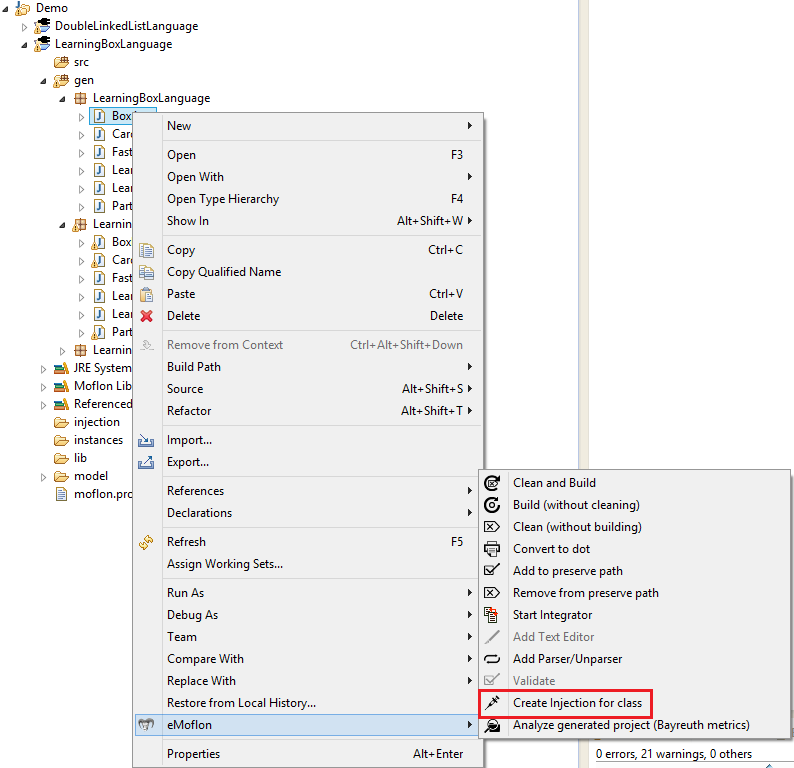
\includegraphics[width=\textwidth]{create_injection_context_menu}
        \caption{Create a new injection}
        \label{fig:injection_create_injection}
    \end{figure}

    This creates a new file in the \texttt{injection} folder of your project with the same packages and name as the Java class but with ``.inject'' as extension
    (Fig. \ref{fig:injection_created_injection_file}). This file contains the definition of a \textit{partial class}~(Fig.~\ref{code:generated_inject_file}) and
    the implementation of the method that was not specified with SDMs.

    \begin{figure}[htbp]
        \centering
        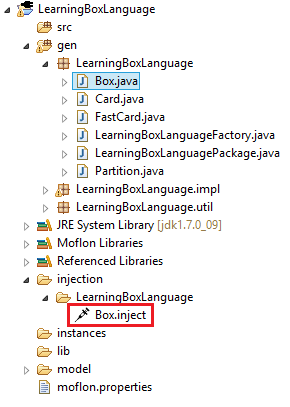
\includegraphics[width=0.54\textwidth]{newly_created_injection_file}
        \caption{Create a new injection}
        \label{fig:injection_created_injection_file}
    \end{figure}
    \FloatBarrier

    \lstdefinelanguage{Injection}[]{Java}{
        morekeywords={partial, class},
        sensitive=false,
        keywordstyle={\bfseries\color{purple}},
        emph={@model},
        emphstyle={\color{blue}},
        backgroundcolor=\color{white}
    }

    \begin{figure}[htbp]
        \centering
        \begin{lstlisting}[language=Injection]
    partial class BoxImpl {

        @model determineNextSize () <--
                // TODO: implement this method here but do not 
                // remove the injection marker
                throw new UnsupportedOperationException();
        -->

        @model addToStringRep (Card card) <--
                StringBuilder sb = new StringBuilder();

                if (stringRep == null)
                {
                    sb.append("BoxContent: [");

                }
                else
                {
                    sb.append(stringRep);
                    sb.append(", [");
                }

                sb.append(card.getFace());
                sb.append(", ");
                sb.append(card.getBack());
                sb.append("]");

                stringRep = sb.toString();
        -->

    }
        \end{lstlisting}
        \caption{Generated injection file}
        \label{code:generated_inject_file}
    \end{figure}
    \FloatBarrier

	\clearpage
    \item[$\blacktriangleright$] You now have the choice of implementing your methods directly in the injection file, or in the corresponding Java file and
    generating the injection from it. We recommend the latter as you can use the usual support from the Java editor. Just don't forget to update the injection
    before re-generating code! Now complete the injection with the code given in Fig. \ref{code:complete_inject_file}.

    \begin{figure}[htbp]
        \centering
        \begin{lstlisting}[language=Injection]
partial class BoxImpl {

    @model determineNextSize () <--

            return getContainedPartition().size() * 10;
    -->

    @model addToStringRep (Card card) <--

            StringBuilder sb = new StringBuilder();

            if (stringRep == null)
            {
                sb.append("BoxContent: [");

            }
            else
            {
                sb.append(stringRep);
                sb.append(", [");
            }

            sb.append(card.getFace());
            sb.append(", ");
            sb.append(card.getBack());
            sb.append("]");

            stringRep = sb.toString();
    -->

}
        \end{lstlisting}
        \caption{Implementation of helper method as an injection}
        \label{code:complete_inject_file}
    \end{figure}
    \FloatBarrier
    \item[$\blacktriangleright$] Rebuild your project (eMoflon $\rightarrow$ Clean and build) and this code will be injected in
    \texttt{LearningBoxLanguage.impl.BoxImpl.java} (Fig. \ref{fig:injected_code_in_boxImpl}). For more information on injections, read
    \ref{sec:appendix_injections}.

\end{enumerate}



    \begin{figure}[htbp]
        \centering
        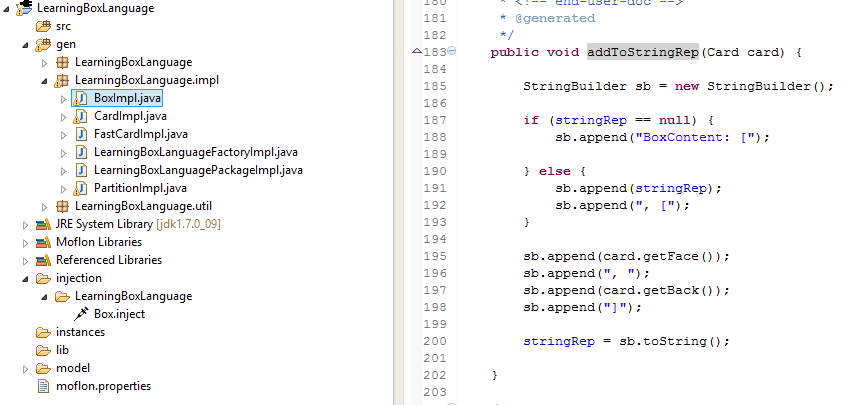
\includegraphics[angle=90,height=0.8\textheight]{injected_code_in_impl}
        \caption{Injected code in BoxImpl after code generation}
        \label{fig:injected_code_in_boxImpl}
    \end{figure}
    
    
{\bf \large this is appendix content. Be sure to review to make sure it flows with the document.}


This chapter describes some extra options when using our injections to integrate handwritten code with generated code. 
This complements the short introduction in Chapter~\ref{sec:intro_injections}.

As an example, we shall provide functionality for saving our \textsf{DoubleLinkedList} to a file.

\begin{enumerate}
  \item[$\blacktriangleright$] Begin with an empty workspace, create a new metamodel \textsf{Demo} and replace the \textsf{Demo.eap} with the file from our .zip
  file (in the folder containing this tutorial).
  \item[$\blacktriangleright$] Now open \textsf{Demo.eap} and change the ``Default Language for Code Generation'' (Tools $\rightarrow$ Options $\rightarrow$
  Source Code Engineering) to \textsf{Ecore}.
  \item[$\blacktriangleright$] Add the method \textsf{void toFile(EString path)} to the class \textsf{List} (Fig.~\ref{fig:append_inj_diagram}) and export the
  project to your Eclipse workspace.
\end{enumerate}
\begin{figure}[htbp]
\begin{center}
  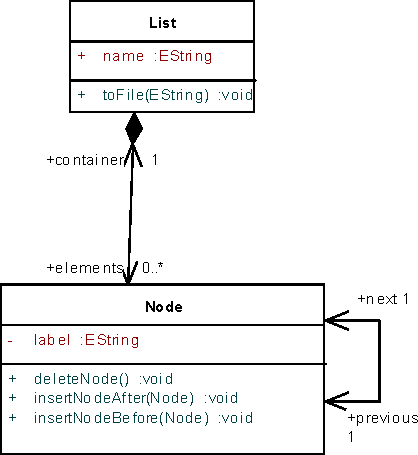
\includegraphics[width=0.5\textwidth]{ea_diagram}
  \caption{Add a new method \textsf{toFile} to the class \textsf{List}}
  \label{fig:append_inj_diagram}
\end{center}
\end{figure}

\begin{enumerate}
  \item[$\blacktriangleright$] Implement the \textsf{toFile} method in \textsf{gen/Double\-Linked\-List\-Language/\-impl/\-ListImpl.java} with the code given in
  Fig. \ref{code:list_toFile_impl_code}.

\begin{figure}[htbp]
\centering
  \begin{lstlisting}[language=Java, keywordstyle={\bfseries\color{purple}}, backgroundcolor=\color{white}]
  public void toFile(String path) {
    // [user code injected with eMoflon]
    try{
      FileWriter fstream = new FileWriter(path);
      BufferedWriter out = new BufferedWriter(fstream);
      out.write(this.toText());
      out.close();
    }catch (Exception e){
      System.err.println(e.toString());
    }
  }
  \end{lstlisting}
\caption{Implementation of \texttt{toFile}}
\label{code:list_toFile_impl_code}
\end{figure}

  \item[$\blacktriangleright$] Right-click \textsf{gen/Double\-Linked\-List\-Language/\-impl/\-ListImpl.java} in the generated Eclipse project and choose
  ``eMoflon/create Injection for class'' to generate the file \textsf{injection/DoubleLinkedListLanguage/\-impl/List\-Impl\-.in\-ject} or update it if it
  already exists. It will contain an injection for the code given in Fig.~\ref{code:list_toFile_impl_code}.
  \item[$\blacktriangleright$] Now rebuild your project (right-click on \texttt{DoubleLinkedListLanguage} and choose ``eMoflon/Build (and clean)'').
  This will rebuild your project and inject the code that we just wrote into \textsf{ListImpl.java}.
  \item[$\blacktriangleright$] You will now find two additional comments just below the imports in the file.
  To generate imports in our injection and get rid of those ``...cannot be resolved'' errors, insert the required imports between the comments as depicted in
  Fig. \ref{code:imports_toFile}.
\begin{figure}[htbp]
\centering
  \begin{lstlisting}[language=Java, keywordstyle={\bfseries\color{purple}}, backgroundcolor=\color{white}]
// <-- [user defined imports]
import java.io.*;
// [user defined imports] -->
  \end{lstlisting}
\caption{Imports for \texttt{toFile}}
\label{code:imports_toFile}
\end{figure}

  \item[$\blacktriangleright$] Now choose ``eMoflon/create Injection for class'' again for \textsf{ListImpl.java} to update the injection file and add the
  imports.

  \item[$\blacktriangleright$] To implement the missing \texttt{toText} method as a \emph{member}, insert the code between the comments at the very end of the
  file as depicted in Fig. \ref{code:toText_impl}

\begin{figure}[htbp]
\centering
  \begin{lstlisting}[language=Java, keywordstyle={\bfseries\color{purple}}, backgroundcolor=\color{white}]
// <-- [user code injected with eMoflon]
private String toText(){
  StringBuilder sb = new StringBuilder();
  for(Node element : elements){
    sb.append(element.getLabel());
    sb.append("\n");
  }
  return sb.toString();
}
// [user code injected with eMoflon] -->
  \end{lstlisting}
\caption{Implementation of \texttt{toText}}
\label{code:toText_impl}
\end{figure}

\end{enumerate}

In this way, member functions and fields that were \emph{not} modelled in EA can be injected using the \texttt{@members} keyword.
Everything between \texttt{<--  -->} is copied into the end of the generated \textsf{ListImpl.java} file without any restrictions at all.

Although it is possible to also inject members in the interface file (i.e., \textsf{List.java} in this example), this is considered dirty and should be used
very sparingly (if possible never).

\fancyfoot[R]{ $\triangleright$ \hyperlink{conclusion}{Next step} } If you ever forget what comments are required to insert imports or code for members, you can
always generate an empty injection and rebuild the project to generate the required comments.

\clearpage